%%This is a very basic article template.
%%There is just one section and two subsections.
\documentclass{article}
\usepackage{amsmath}
\usepackage{float}
\usepackage{graphicx}

\begin{document}
\newcommand{\bx}{\mathbf{x}}
\newcommand{\ddq}{\frac{\partial}{\partial \epsilon_t}}
\newcommand{\dxdq}{\frac{\partial \bx}{\partial \epsilon_t}}

\section{Dense 3D Reconstruction using Robot Hand-Mounted Cameras}

This is a general sketch of an idea for reconstructing a dense 3D scene using a
hand-mounted depth camera.

\subsection{Problem}

Consider a robot that has a configuration space $C \subseteq \mathbf{R}^N$.
Mounted on one of the links of the robot is a depth sensor. The task is, given a
sequence of noisy configurations at each time step $\{q_1, q_2, \ldots,
q_T\}$, and a sequence of noisy sensor readings (point clouds) captured
simultaneously $\{Z_1, Z_2, \ldots, Z_T\}$, where $Z_i = \{\bx_1, \ldots, x_N\}
\subseteq \mathbf{R}^3$, reconstruct the true dense 3D geometry of the scene. 

\subsection{World Representation}

We will represent the world as a truncated signed distance function (TSDF). It
is defined as $D(\bx) : \mathbf{R}^3 \to \mathbf{R}$, and represents the
(signed) distance to the nearest obstacle in meters, up to a truncation distance $\tau$.

The gradient of the distance field $\nabla D : \mathbf{R}^3 \to \mathbf{R}^3$,
is clearly defined and easy to compute.

\subsection{General Approach}

We will iteratively build up the TSDF. $D_t$ is calculated by first estimating a
configuration of the robot $q^*_t = q_t + \epsilon^*_t$ which minimizes the
squared error between the sensor measurements $Z_t$ and the previous TSDF model
$D_{t - 1}$.  Then, the sensor measurements are projected back into the world
given $q^*_t$, and the usual TSDF update is applied.

\begin{figure}
	\centering
	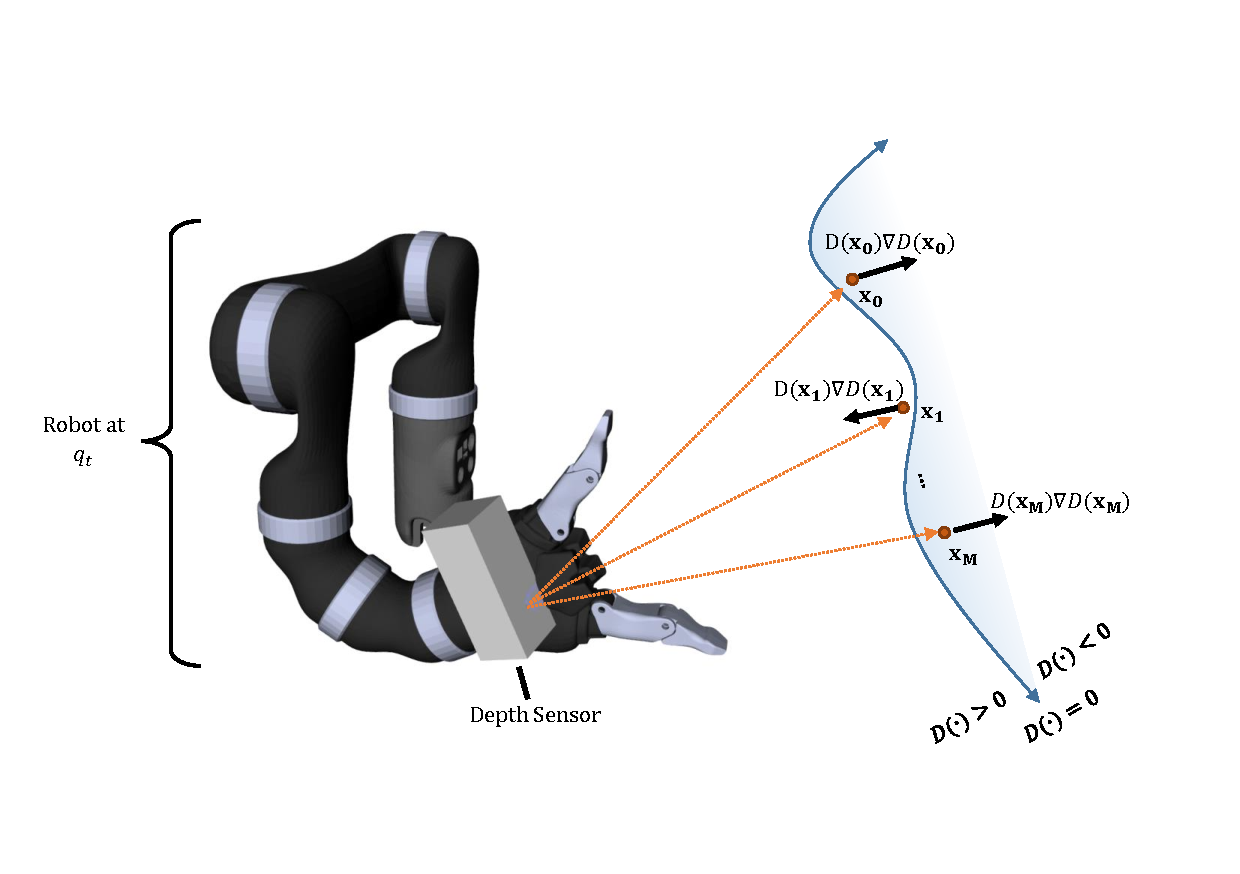
\includegraphics[width=1.0\textwidth]{img/robot_reconstruct.pdf}
	\caption{A diagram of the robot sensing a surface with a depth sensor. Rays
	from the depth sensor are shown as orange dotted lines. The point cloud
	$\{\bx_1, \ldots, \bx_M\}$ is used to determine the gradient of the distance
	field $\nabla D$ at each point.}
	\label{fig:robot} 
\end{figure}

\subsection{Noise Model} 

The robot's configuration at time step $t$ is given by joint encoder readings
$q_t$, which is a random value drawn from the distribution:

$$q_t = q_t^{\text{true}} + \epsilon_t$$

\noindent Where $q_t^{\text{true}}$ are the true joint angles of the robot,
and $\epsilon_t$ is a random offset drawn from some unknown random distribution
$Q$.

$$ \epsilon_t \sim Q(q_t^{\text{true}}) $$

In practice, $Q$ is highly nonlinear, and depends on the dynamics of the
system (for example, the direction of gravity, or other factors that depend
on the robot's joint angles). Therefore, finding an \emph{a. priori}
represention of $Q$ may be infeasible. The task is to compute $\epsilon^*_t$, which is an estimate of the
current noisy offset.

\subsection{Computing $\epsilon^*_t$}

We can compute $\epsilon^*_t$ by performing \textbf{gradient descent} in the
configuration space of the robot.  Define the \textbf{forward kinematics
function} $F(q_t, Z_t) : \mathbf{R}^3 \to \mathbf{R}^3$, which merely
transforms the point cloud $Z_t$ into the world frame, given configuration $q_t
\in C$. Call

$$ F_t = F(q_t + \epsilon_t, z_t) $$

Then, the objective function $h(\epsilon_t, D_{t-1}) : C \to \mathbf{R}$ is
given by the sum squared distances of all of the projected points in $F_t$:

$$ h(\epsilon_t, D_{t-1}) = \sum_{x \in F_t}\left(D_{t-1}(x)\right) ^2 $$

\subsubsection{Computing the Gradient}

Now, we want to find the partial differential of $h$ with respect to
$\epsilon_t$:


\begin{align} 
\frac{\partial{h}}{\partial{\epsilon_t}} &= \ddq  \sum_{\bx
\inF_t}\left(D_{t-1}(\bx)\right) ^2 \\ &= \sum_{\bx \inF_t} \ddq
\left(D_{t-1}(\bx)\right) ^2 \\ &=\text{Making use of the chain rule? Since \bx
is a function of~} q_t \ldots \\ &= 2\sum_{\bx \in F_t} D_{t-1}(\bx) \dxdq \nabla
D_{t-1}(\bx)
\end{align}

And, since $\dxdq$ is the change in $\bx$, a projected sensor point, with
respect to $\epsilon_t$, the configuration of the robot at time $t$, we have (with some
handwaving):

$$ \dxdq = J_\bx \in \mathbf{R}^{3 \times N}$$

Where $J_\bx$ is the serial manipulator Jacobian computed for
the point $\bx$, as though it were rigidly attached to the manipulator by
the ray connecting $\bx$ to the sensor. $J$ has the form:

\begin{equation} J_\bx = \left[
\begin{array}{ccc}
| & \ldots & | \\
\frac{\partial \bx}{\partial \epsilon_t(1)} & \ldots & \frac{\partial
\bx}{\partial \epsilon_t(N)}  \\
| & \ldots & |
\end{array}
\right]
\end{equation}

\noindent And so:

$$ \frac{\partial{h}}{\partial{\epsilon_t}} = 2\sum_{x \in F_t} D_{t-1}(x)
{\mathbf{J}_x}^{\text{T}} \nabla D_{t-1}(x) $$

\noindent We will call this quantity $\nabla h(\epsilon_t)$. It has a nice physical
interpretation: imagine all the points in the point cloud are attached rigidly
to the robot manipulator on rods. At then end of each rod $x$, apply a force
$D_{t - 1}(x) \nabla D_{t -1} (x)$. The resulting torque on the robot's joints 
is proportional to $\nabla h(\epsilon_t)$ by a factor of 2 (Fig. \ref{fig:robot}).

\subsubsection{Gradient Descent}

Now, we just follow the update rule, setting ${\epsilon_t}^{(0)} =
\epsilon_{t - 1}$:

$$ {\epsilon_t}^{(i + 1)} = {\epsilon_t}^{(i)} - \lambda \nabla
h(\epsilon_t^{(i)}) $$

\noindent Where $\lambda$ is a learning rate. We follow the gradient until
convergence, yielding $\epsilon^*_t$, treating the joint limits of the robot as
a constraint.


\end{document}
